\section{Numerical Experiments}

\subsection{Refinement/Coarsening Convergence Test}

\begin{figure}
    \centering
    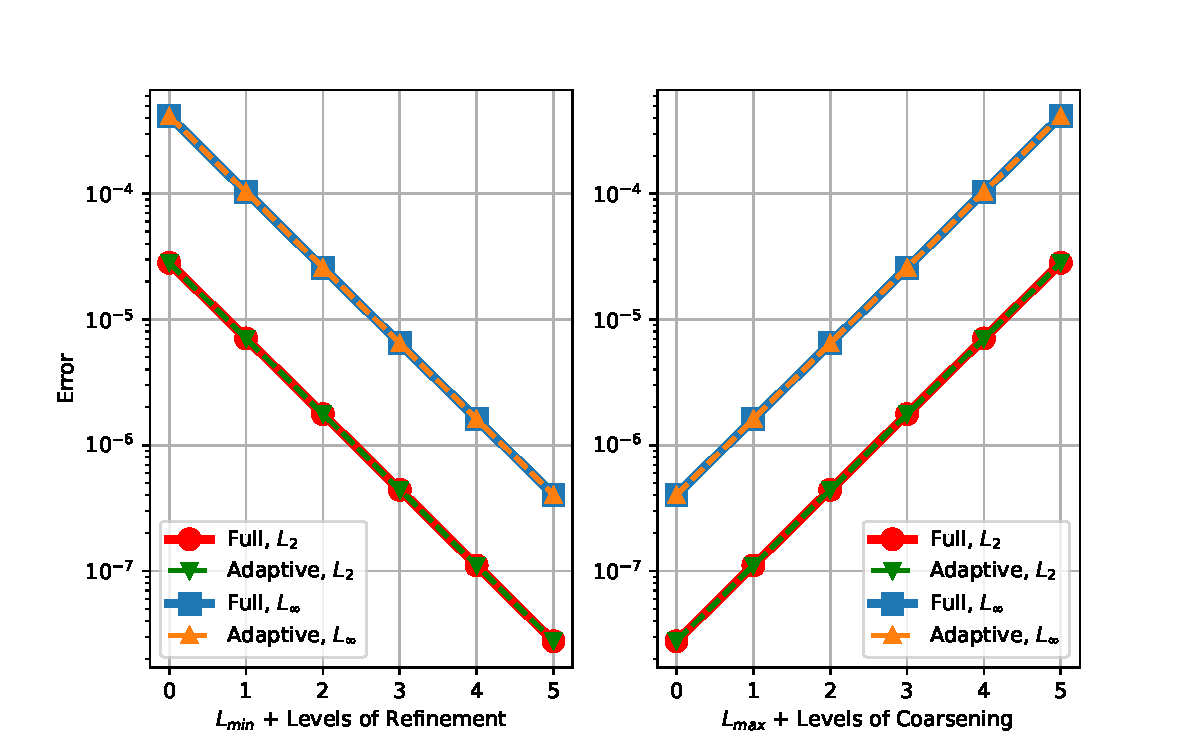
\includegraphics[width=\textwidth, clip=true, trim={40 0 40 40}]{figures/full-vs-adaptive-convergence-no-title.pdf}
    \caption{[TODO]}
    \label{fig:full-vs-adaptive-convergence}
\end{figure}

\subsection{Random Refinement}

\begin{figure}
    \centering
    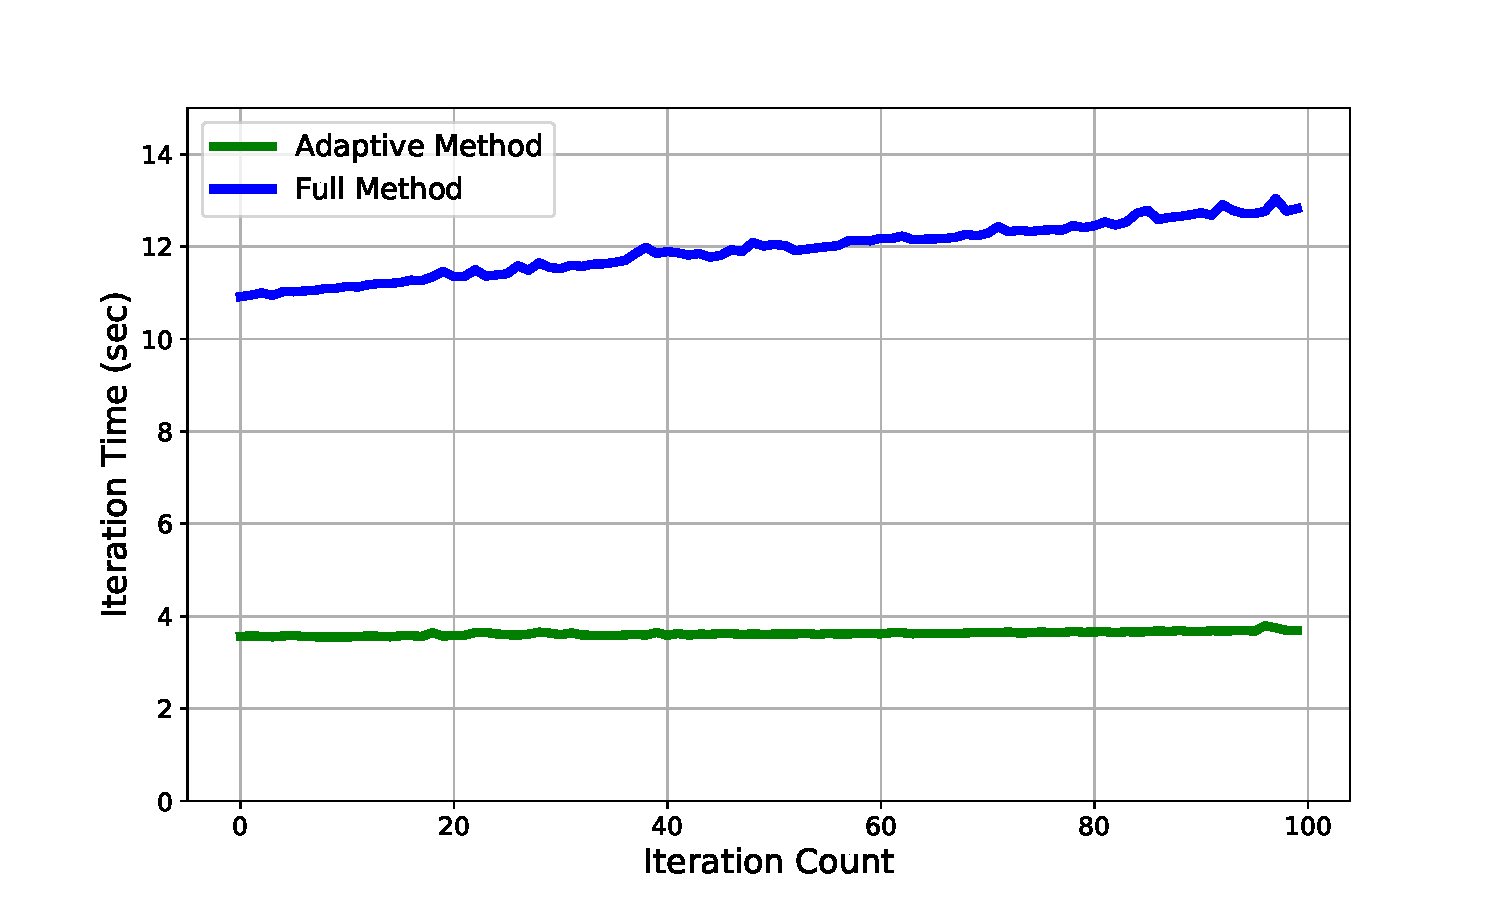
\includegraphics[width=\textwidth, clip=true, trim={40 0 40 40}]{figures/full-vs-adaptive-time-comparison-no-title.pdf}
    \caption{[TODO]}
    \label{fig:full-vs-adaptive-time-comparison}
\end{figure}

\begin{figure}
    \centering
    \begin{subfigure}[t]{1\textwidth}
        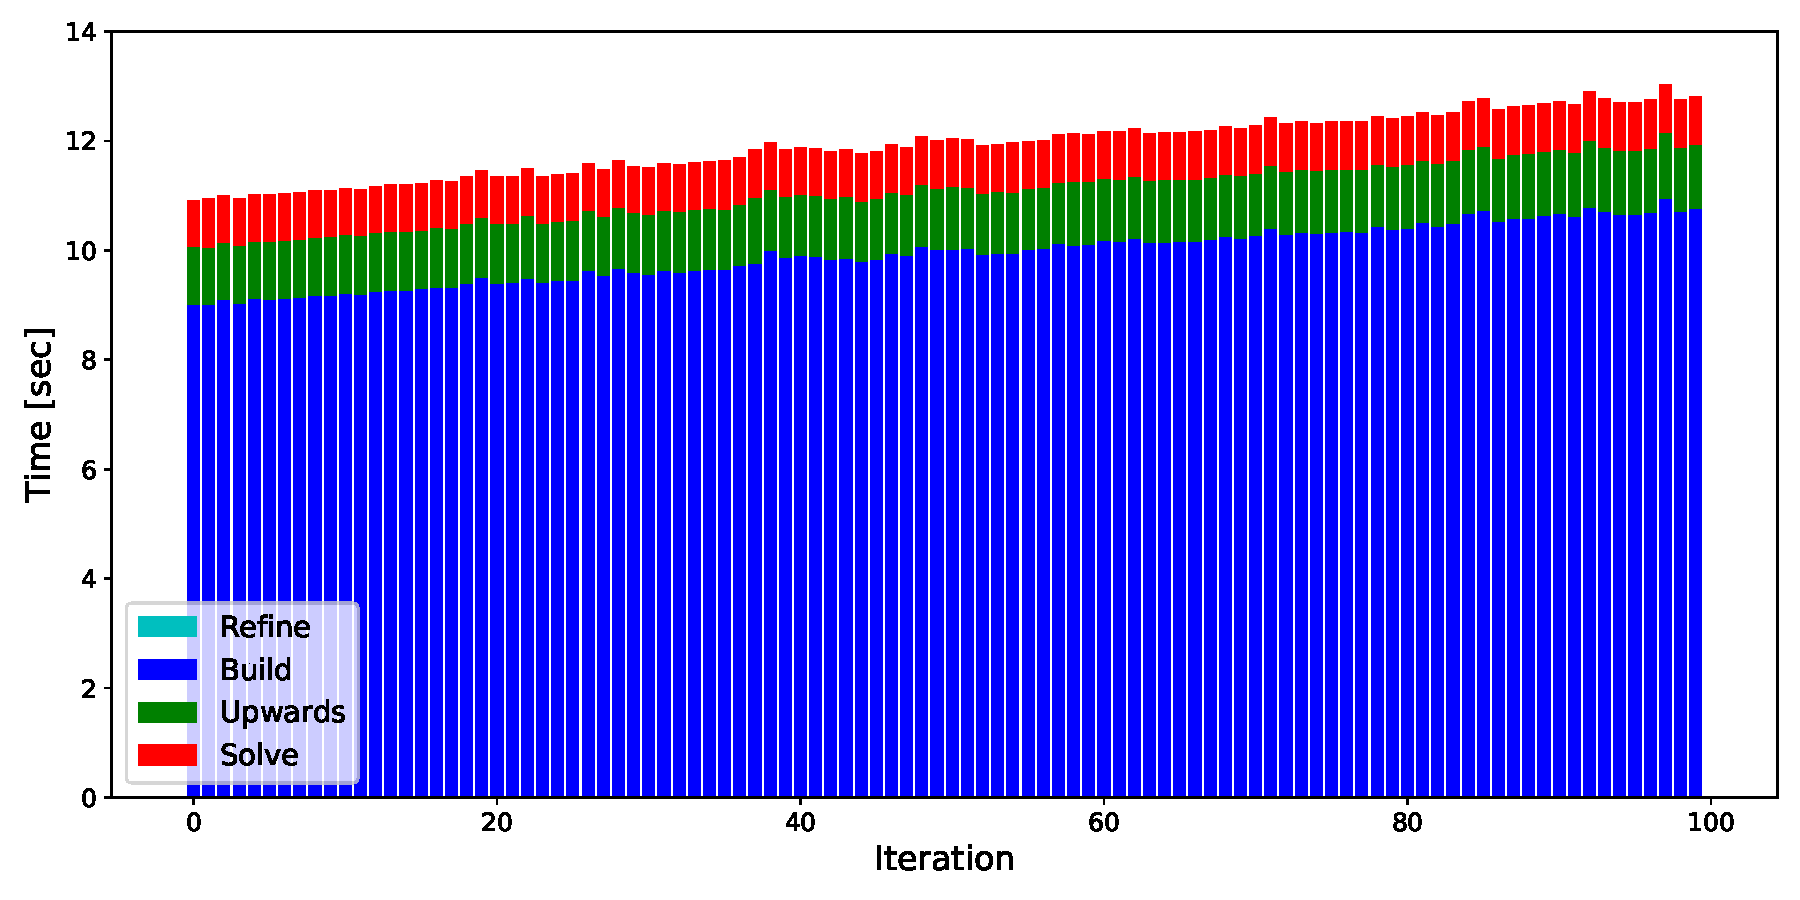
\includegraphics[width=\textwidth, clip=true, trim={10 10 10 10}]{figures/full-stacked-bar-no-title.pdf}
        \caption{Full build method}
    \end{subfigure}
    \begin{subfigure}[t]{1\textwidth}
        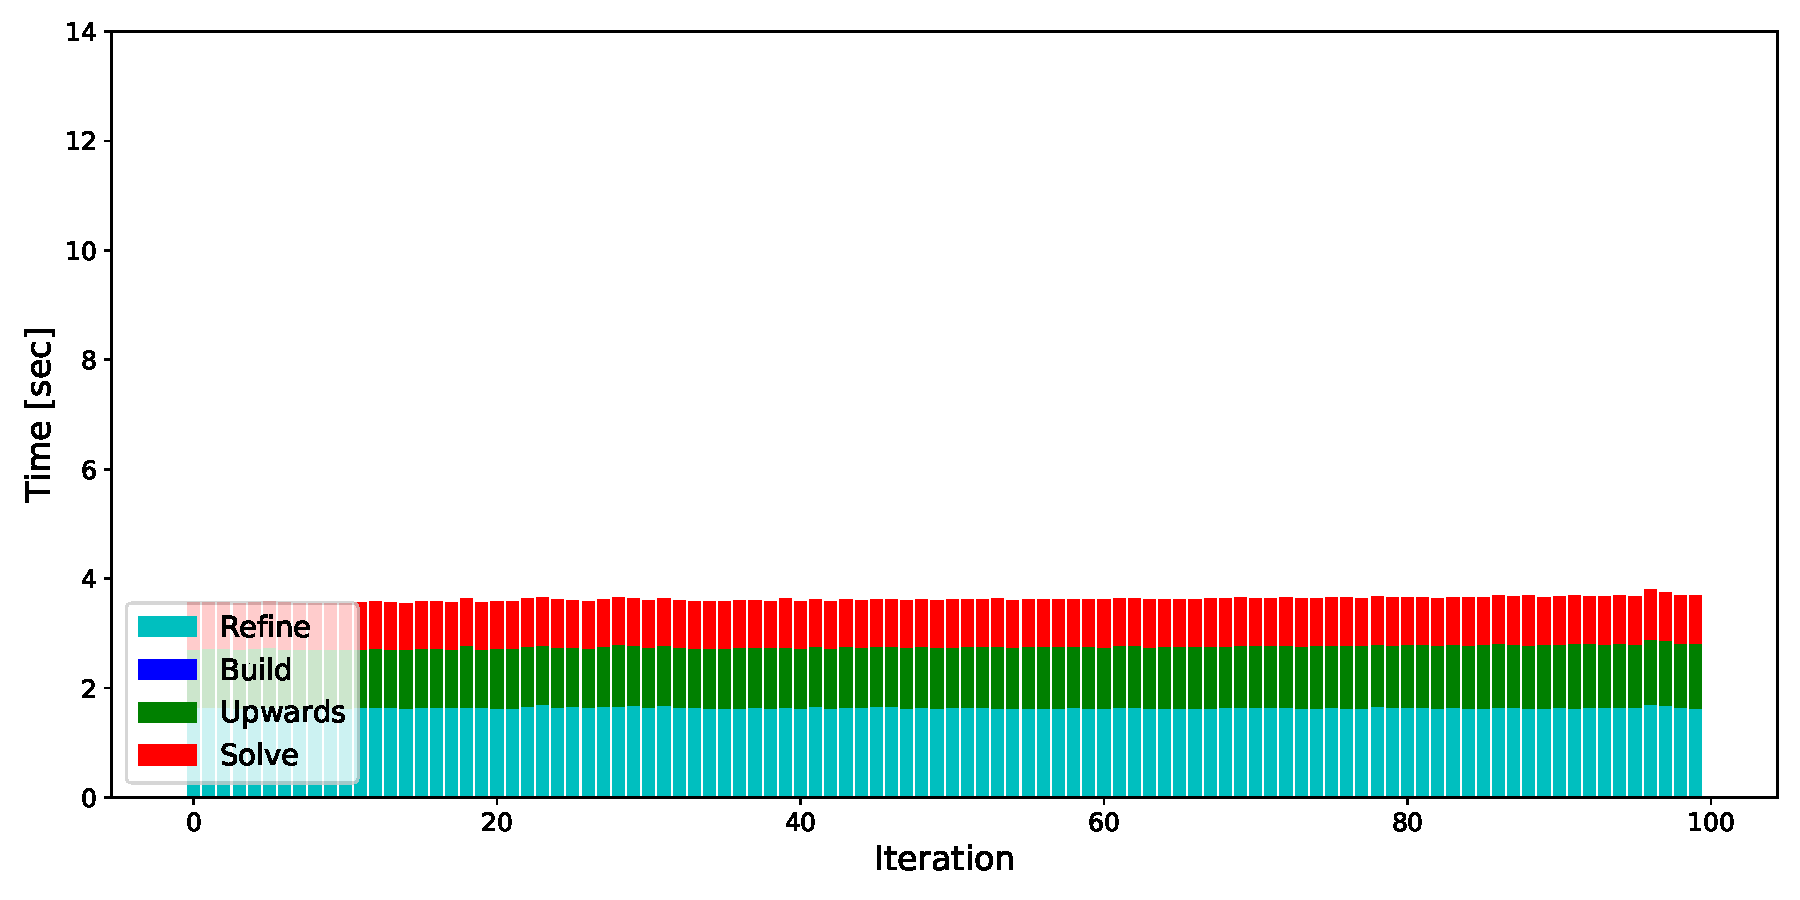
\includegraphics[width=\textwidth, clip=true, trim={10 10 10 10}]{figures/adaptive-stacked-bar-no-title.pdf}
        \caption{Adaptive build method}
    \end{subfigure}
    \caption{Comparison of full vs. adaptive build methods for the random refinement experiment. In each iteration, a random leaf node is refined and the elliptic problem is solved with the QAHPS method. Note the scale of the y-axis in both plots.}
    \label{fig:full-vs-adaptive-time-comparison}
\end{figure}